\documentclass[border=4pt]{standalone}
% shared style for all PyTBA topology diagrams (\input by each standalone file)
\usepackage{mathpazo}
\usepackage{amsmath}
\usepackage{tikz}
\usetikzlibrary{positioning,arrows.meta,calc,decorations.pathreplacing,fit,backgrounds}
\tikzset{
  host/.style={draw=blue!55!black, fill=blue!7, rounded corners=2pt, align=center,
               minimum height=9mm, minimum width=22mm, font=\small},
  blk/.style={draw=black!60, fill=black!4, rounded corners=2pt, align=center,
              minimum height=8mm, font=\small},
  chan/.style={draw=orange!70!black, fill=orange!8, rounded corners=2pt, align=center,
               minimum height=9mm, font=\small},
  lossbox/.style={draw=red!70!black, fill=red!6, rounded corners=2pt, align=center, font=\footnotesize},
  data/.style={-{Stealth[length=2.2mm]}, thick},
  ack/.style={-{Stealth[length=2mm]}, dashed, black!60},
  lbl/.style={font=\footnotesize, align=center},
  brace/.style={decorate, decoration={brace, amplitude=4pt}, thick, black!70},
}

\begin{document}
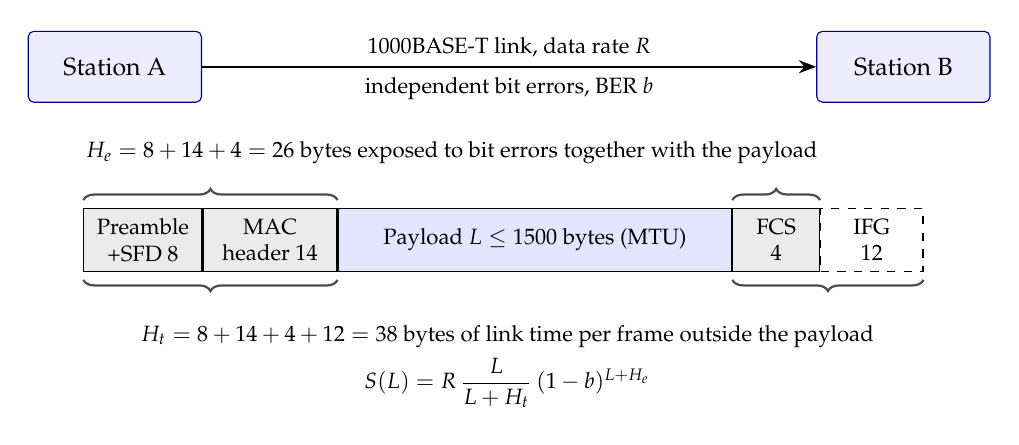
\begin{tikzpicture}
\node[host] (a) {Station A};
\node[host, right=78mm of a] (b) {Station B};
\draw[data] (a) -- node[lbl, above] {1000BASE-T link, data rate $R$} node[lbl, below] {independent bit errors, BER $b$} (b);
% frame layout
\begin{scope}[yshift=-22mm, xshift=-4mm, every node/.style={draw, minimum height=8mm, font=\footnotesize, align=center, inner sep=1pt}]
\node[fill=black!8, minimum width=15mm, anchor=west] (pre) at (0,0) {Preamble\\+SFD 8};
\node[fill=black!8, minimum width=17mm, right=0mm of pre] (hdr) {MAC\\header 14};
\node[fill=blue!10, minimum width=50mm, right=0mm of hdr] (pay) {Payload $L \le 1500$ bytes (MTU)};
\node[fill=black!8, minimum width=11mm, right=0mm of pay] (fcs) {FCS\\4};
\node[fill=white, dashed, minimum width=13mm, right=0mm of fcs] (ifg) {IFG\\12};
\end{scope}
\draw[brace] ($(pre.north west)+(0,1mm)$) -- ($(hdr.north east)+(0,1mm)$);
\node[lbl] at ($(pre.north west)!0.5!(fcs.north east)+(0,7mm)$) {$H_e=8+14+4=26$ bytes exposed to bit errors together with the payload};
\draw[brace] ($(fcs.north west)+(0,1mm)$) -- ($(fcs.north east)+(0,1mm)$);
\draw[brace, decoration={mirror, amplitude=4pt}] ($(pre.south west)+(0,-1mm)$) -- ($(hdr.south east)+(0,-1mm)$);
\draw[brace, decoration={mirror, amplitude=4pt}] ($(fcs.south west)+(0,-1mm)$) -- ($(ifg.south east)+(0,-1mm)$);
\node[lbl] at ($(pre.south)!0.5!(ifg.south)+(0,-12mm)$) {$H_t=8+14+4+12=38$ bytes of link time per frame outside the payload\\[1mm] $S(L)=R\,\dfrac{L}{L+H_t}\,(1-b)^{L+H_e}$};
\end{tikzpicture}
\end{document}
